\chapter{Metodologia}
\label{cap:metodologia}

Este capítulo apresenta o percurso metodológico estruturado para conduzir a pesquisa, conectando a proposta teórica do ElicitBot à sua execução prática. O texto abrange desde o detalhamento das fases cronológicas de diagnóstico, refatoração, validação empírica e análise de resultados, até a fundamentação do paradigma científico e das práticas de Engenharia de Software adotadas para reger o desenvolvimento do artefato.

\section{Design da Pesquisa}
\label{sec:design_pesquisa}

Este estudo caracteriza-se como uma pesquisa aplicada, com abordagem mista (quali-quantitativa), focada na viabilização de uma ferramenta de software educacional para apoio ao ensino na disciplina de Requisitos de Software. O ciclo de evolução do sistema adota princípios complementares de Engenharia de Software Orientada a Dados (\textit{Data-Driven Development}) \cite{olsson2014}, utilizando métricas de uso e \textit{feedbacks} dos estudantes para realizar o seu refinamento iterativo.

O \textit{design} da pesquisa foi estruturado em quatro fases sequenciais e complementares, projetadas para atender aos cinco objetivos específicos do estudo: (1) Diagnóstico e Planejamento; (2) Refatoração e Desenvolvimento; (3) Implantação e Validação em Campo; e (4) Avaliação e Análise de Resultados. A Figura \ref{fig:fases_pesquisa} demonstra o encadeamento lógico dessas fases ao longo da pesquisa.

\begin{figure}[H]
    \centering
    \caption{Fluxograma de Fases da Pesquisa}
    \label{fig:fases_pesquisa}
    
    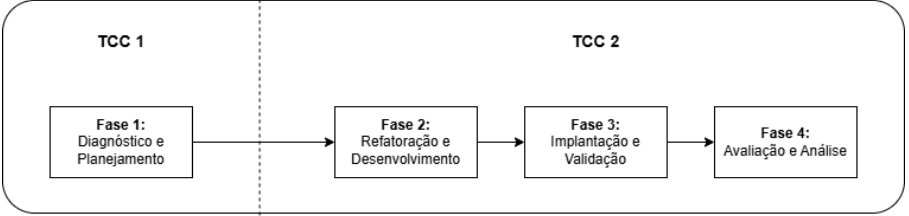
\includegraphics[width=0.9\textwidth]{figuras/fases_pesquisa.png}
    
    \small Fonte: Elaborada pelo autor.
\end{figure}

A Tabela \ref{tab:objetivos_metodos} relaciona as fases do projeto aos seus respectivos Objetivos Específicos (OE), detalhando as atividades executadas para alcançá-los, os métodos e procedimentos técnicos aplicados, além dos resultados esperados para cada etapa.

\noindent
{
\footnotesize 
\renewcommand{\arraystretch}{1.1}
\setlength{\LTleft}{0pt}
\setlength{\LTright}{0pt}

\begin{xltabular}{\textwidth}{|p{1.8cm}|p{4.2cm}|X|X|X|}
    \caption{Objetivos, atividades, métodos e resultados esperados} \label{tab:objetivos_metodos} \\
    \toprule
    \textbf{Fase da Pesquisa} & \textbf{Objetivos Específicos (OE)} & \textbf{Atividades} & \textbf{Métodos Aplicados} & \textbf{Resultados Esperados} \\
    \midrule
    \endfirsthead

    \multicolumn{5}{c}%
    {{\bfseries \tablename\ \thetable{} -- continuação da página anterior}} \\
    \toprule
    \textbf{Fase da Pesquisa} & \textbf{Objetivos Específicos (OE)} & \textbf{Atividades} & \textbf{Métodos Aplicados} & \textbf{Resultados Esperados} \\
    \midrule
    \endhead

    \midrule \multicolumn{5}{r}{{Continua na próxima página...}} \\
    \endfoot

    \bottomrule
    \multicolumn{5}{c}{\small Fonte: Elaborada pelo autor.} \\
    \endlastfoot
    
    % --- FASE 1 ---
    \textbf{Fase 1: Diagnóstico e Planejamento} & 
    (OE1) Diagnosticar o estado atual do ElicitBot, mapeando seu escopo funcional, limitações de implementação e gargalos arquiteturais. & 
    A1.1: Análise do trabalho acadêmico original e do código-fonte herdado. & 
    Revisão Documental e Inspeção de Código. & 
    Mapeamento do escopo funcional da ferramenta. \\
    \cline{3-5} 
    
    & & 
    A1.2: Levantamento e identificação de gargalos arquiteturais e de escalabilidade. & 
    Entrevista Semiestruturada e Análise de Débito Técnico. & 
    Diagnóstico das limitações de implementação e gargalos arquiteturais. \\
    \cline{2-5} 
    
    & 
    (OE2) Estruturar o plano de evolução técnica e funcional do ElicitBot, contemplando as estratégias de mitigação arquitetural e a especificação do \textit{backlog} priorizado para uso em turma. & 
    A2.1: Definição de estratégias para mitigar as limitações de escalabilidade. & 
    Análise de Viabilidade Técnica. & 
    Plano de evolução técnica documentado por Registros de Decisão (ADR) e \textit{Backlog}. \\
    \cline{3-5} 
    
    & & 
    A2.2: Especificação e priorização do \textit{backlog} de evolução funcional. & 
    Engenharia de Requisitos Ágil e Priorização MoSCoW. & 
    Documento de \textit{Product Backlog} priorizado. \\
    \midrule
    
    % --- FASE 2 ---
    \textbf{Fase 2: Refatoração e Desenvolvimento} & 
    (OE3) Implementar a evolução técnica e funcional do ElicitBot, visando torná-lo viável, estável e escalável para aplicação em cenários educacionais reais. & 
    A3.1: Implementação do plano de ação para resolver os problemas de escalabilidade. & 
    Refatoração de Software. & 
    Evolução técnica implementada (arquitetura viável e escalável). \\
    \cline{3-5}
    
    & & 
    A3.2: Desenvolvimento das melhorias funcionais priorizadas. & 
    Desenvolvimento Incremental. & 
    Incremento de software contendo a evolução funcional da ferramenta. \\
    \cline{3-5}
    
    & & 
    A3.3: Execução de testes técnicos para validação de estabilidade estrutural. & 
    Testes de Carga em Degraus (\textit{Step Load}) e Testes de Resistência (\textit{Soak Test}). & 
    Validação de desempenho e estabilidade estrutural sob concorrência. \\
    \midrule
    
    % --- FASE 3 ---
    \textbf{Fase 3: Implantação e Validação em Campo} & 
    (OE4) Validar a ferramenta em sessão prática com alunos da disciplina Requisitos de Software, coletando dados de uso e percepção dos estudantes para apoiar o seu refinamento. & 
    A4.1: Implantação e aplicação do sistema em sala de aula. & 
    Teste de Aceitação do Usuário (UAT). & 
    Ambiente operacional validado e sessão prática executada. \\
    \cline{3-5}
    
    & & 
    A4.2: Coleta de métricas de uso e aplicação do questionário de avaliação. & 
    Instrumentação de Software (\textit{Logs}) e Questionário de Avaliação Estruturado. & 
    Registros de interação e base de dados de percepção dos estudantes. \\
    \cline{3-5}
    
    & & 
    A4.3: Análise qualitativa dos relatos e sistematização do plano de ação. & 
    Triagem Técnica de Incidentes e Categorização de Relatos. & 
    Diagnóstico qualitativo e plano de ação estruturado para o refinamento. \\
    \cline{3-5}
    
    & & 
    A4.4: Aplicação das correções imediatas para refinamento do sistema. & 
    Manutenção Corretiva e Evolutiva de Software. & 
    Refinamento da ferramenta com correções imediatas aplicadas. \\
    \midrule
    
    % --- FASE 4 ---
    \textbf{Fase 4: Avaliação e Análise de Resultados} & 
    (OE5) Avaliar as vantagens, limitações e desafios do uso de \textit{chatbots} baseados em LLMs no apoio ao aprendizado prático de Engenharia de Requisitos. & 
    A5.1: Consolidação, higienização e apuração estatística dos dados quantitativos. & 
    Alfa de Cronbach, Análise de Funil, Estatística Descritiva e Análise de Sensibilidade. & 
    Indicadores estatísticos consolidados por critério e dimensão avaliada. \\
    \cline{3-5}
    
    & & 
    A5.2: Triangulação dos resultados quantitativos e qualitativos da validação. & 
    Triangulação Metodológica (Análise Quali-Quanti). & 
    Síntese integrada das vantagens, limitações e potencial de adoção da ferramenta. \\
    \cline{3-5}
    
    & & 
    A5.3: Análise comparativa da evolução técnica e funcional da ferramenta. & 
    Análise Comparativa Multicritério. & 
    Comparativo sistemático entre a prova de conceito original e a versão evoluída. \\
\end{xltabular}
}

\section{O Paradigma da \textit{Design Science Research}}
\label{sec:dsr}

A investigação em Engenharia de Software e Sistemas de Informação exige, frequentemente, abordagens que vão além da descrição ou explicação de fenômenos, orientando-se para a resolução ativa de problemas reais. Nesse contexto, para reger as fases de \textit{design} descritas na seção anterior, o presente trabalho adota como base metodológica a \textit{Design Science Research} (DSR). Segundo \citeonline{hevner2004}, a DSR é um paradigma centrado na criação e avaliação iterativa de um artefato inovador de Tecnologia da Informação (TI), concebido para solucionar problemas organizacionais ou educacionais específicos, gerando simultaneamente conhecimento científico válido.

O rigor e a aplicabilidade desta metodologia são assegurados pela interação contínua entre três ciclos metodológicos fundamentais propostos por \citeonline{hevner2007}:

\begin{itemize}
    \item \textbf{Ciclo de Relevância (\textit{Relevance Cycle}):} Estabelece a ponte entre o ambiente prático e a investigação (Fases 1 e 4 do projeto). No escopo deste estudo, o ambiente é o contexto educacional do ensino de Requisitos de Software, onde a dificuldade de pôr em prática o conhecimento teórico adquirido pelos estudantes representa o problema real a ser resolvido.
    \item \textbf{Ciclo de Rigor (\textit{Rigor Cycle}):} Conecta a pesquisa à base de conhecimento científico pré-existente (Fases 1 e 4). Para a evolução e avaliação do sistema, este ciclo é garantido pela aplicação de métodos consolidados de Engenharia de Software (como técnicas de refatoração de código, testes de carga e instrumentação de \textit{logs}), análise estatística e pela literatura especializada para fundamentar as decisões arquiteturais e a interpretação dos dados.
    \item \textbf{Ciclo de Design (\textit{Design Cycle}):} Constitui o núcleo empírico do método, operando como o motor iterativo de construção e avaliação (Fases 2 e 3). Neste trabalho, este ciclo consiste no desenvolvimento das melhorias do software, nos testes de estresse sob concorrência, na sessão prática de validação com os alunos e na aplicação de correções direcionadas pelos dados coletados.
\end{itemize}

Nesta estrutura de investigação, o ElicitBot atua como o artefato central da DSR. A conexão entre as quatro fases operacionais e os ciclos metodológicos garante que a versão final do sistema não apenas cumpra a sua utilidade pedagógica de forma estável, mas também contribua com evidências científicas sólidas sobre o uso de Inteligência Artificial no apoio ao ensino superior.

\section{Práticas de Engenharia de Software}
\label{sec:pra_eng_soft}

O projeto adotou uma metodologia ágil híbrida baseada em \textit{Scrumban}, estruturando o ciclo de vida em \textit{Sprints} iterativas e gerenciando o fluxo de tarefas visualmente por meio de um quadro \textit{Kanban} \cite{scrumstudy2024}. A gestão de escopo utilizou Histórias de Usuário priorizadas pelo método MoSCoW \cite{agilebusiness2014}. Para garantir a qualidade técnica, a escalabilidade e a manutenibilidade do software, o processo foi complementado por práticas de engenharia derivadas do \textit{eXtreme Programming} (XP) e da arquitetura de software moderna:

\begin{itemize}
    \item \textbf{Padrões Arquiteturais e de Projeto (\textit{Design Patterns}):} Adotou-se uma Arquitetura em Camadas (\textit{Layered Architecture}) desacoplada via API RESTful \cite{pressman2021, martin2018}. No servidor, aplicaram-se os padrões \textit{Repository Pattern} (para abstração da persistência relacional assíncrona via ORM), \textit{Service Layer} \cite{fowler2002} (para isolamento das regras de negócio e orquestração do modelo de linguagem), \textit{Dependency Injection} (para gestão de sessões de banco de dados, autenticação e controle de acesso) e \textit{Fallback Strategy} (para degradação graciosa em caso de falhas no uso de cache na nuvem).
    \item \textbf{Qualidade de Código e Contratos Estritos:} Aplicaram-se práticas de Refatoração Contínua \cite{fowler2020}, \textit{Design} Simples e padronização rigorosa de código com tipagem estrita e validação automatizada de esquemas (\textit{Data Transfer Objects} -- DTOs) nas fronteiras entre o cliente, o servidor e a API de Inteligência Artificial, aliadas ao controle de versão por \textit{conventional commits} e conteinerização com Docker.
    \item \textbf{Verificação, Testes de Carga e Validação:} A estratégia de testes abrangeu: (i) validação determinística de integridade de dados e esquemas no \textit{backend}; (ii) Testes de Carga em Degraus (\textit{Step Load Testing}) e Testes de Resistência (\textit{Soak Testing}) automatizados via ferramenta \textit{Locust} para aferir o comportamento assíncrono do servidor e do \textit{pool} de conexões sob estresse; e (iii) Teste de Aceitação do Usuário (UAT) \cite{sommerville2016} em sala de aula.
\end{itemize}

\section{Ferramentas de Apoio e Uso de Inteligência Artificial Generativa}
\label{sec:uso_ia}

Para viabilizar a execução estruturada dos ciclos metodológicos detalhados anteriormente, a pesquisa contou com suporte tecnológico contínuo. Dessa forma, em conformidade com as diretrizes de integridade na pesquisa científica estabelecidas pela Portaria CNPq Nº 2.664/2026, declara-se o uso de ferramentas de Inteligência Artificial Generativa (IAG) como instrumento de apoio metodológico, analítico e operacional durante a elaboração deste Trabalho de Conclusão de Curso.

Especificamente, foram utilizadas as ferramentas NotebookLM e Gemini (Google). Na elaboração documental, essas tecnologias atuaram como suporte nas fases de pesquisa bibliográfica, cruzamento de referências teóricas, revisão gramatical, geração de representações gráficas, formatação do código em \LaTeX\ e sumarização da transcrição da entrevista semiestruturada realizada com o desenvolvedor original do sistema herdado. No âmbito de engenharia e análise de dados, o Gemini foi utilizado como ferramenta de assistência no desenvolvimento e refatoração do código-fonte da aplicação (\textit{frontend} e \textit{backend}) e na escrita dos scripts de testes de carga, bem como no apoio à identificação de gargalos operacionais e tabulação dos dados coletados.

Ressalta-se que nenhuma ferramenta de IAG foi utilizada para a geração autônoma de conteúdo ou de código sem supervisão. Todo o código-fonte sugerido passou por revisão crítica, adaptação e validação funcional rigorosa por parte do autor. Do mesmo modo, a tomada de decisão documentada nos Registros de Decisão Arquitetural (ADRs), o planejamento descrito nos \textit{Backlogs} Técnico e Funcional, a interpretação crítica dos dados coletados e a redação final do texto são de autoria intelectual exclusiva do pesquisador. Dessa forma, o autor assume responsabilidade integral sobre o conteúdo final deste documento e do software produzido, garantindo a sua originalidade, veracidade e a devida mitigação de eventuais imprecisões ou plágios, em estrito cumprimento às exigências éticas da Política de Integridade na Atividade Científica do CNPq.

\section{Fase 1: Diagnóstico e Planejamento}
\label{sec:fase1}

Estabelecidas as bases teóricas do paradigma adotado e os instrumentos de apoio metodológico, a execução prática do projeto teve início na Fase 1. Esta etapa objetivou diagnosticar o estado original da prova de conceito ElicitBot e planejar estruturalmente a sua evolução tecnológica e funcional. Para garantir um fluxo lógico, essa fase foi subdividida em dois objetivos sequenciais, que conectaram a compreensão da arquitetura herdada à proposição de soluções viáveis para a implantação em ambiente educacional.

\subsection{(A1.1) Análise do trabalho acadêmico original e do código-fonte herdado}

A primeira atividade (A1.1) concentrou-se em compreender a fundamentação e a estrutura interna do ElicitBot original. Para isso, foi realizada a Revisão Documental sobre o trabalho de \citeonline{junior2025}, adotando uma leitura direcionada aos capítulos de especificação e validação para extrair o escopo de requisitos e o contexto das decisões de \textit{design} iniciais. Paralelamente, foi conduzida uma Inspeção Estática de Código, realizada diretamente na interface do repositório remoto (GitHub\footnote{GitHub. Documentação Oficial. Disponível em: \url{https://docs.github.com/}. Acesso em: 18 jun. 2026.}) herdado. Essa verificação rastreou o fluxo de execução das classes controladoras (como a gestão do modelo de linguagem), a lógica de engenharia de \textit{prompts} e o ciclo de vida das requisições HTTP.

O uso integrado dessas práticas é recomendado na literatura para a detecção precoce de anomalias e entendimento estrutural amplo antes de qualquer processo de refatoração \cite{sommerville2016}. Como resultado direto desta atividade, buscou-se consolidar o mapeamento formal do escopo funcional da ferramenta em sua versão inicial, fornecendo a base técnica necessária para o levantamento de seus requisitos de evolução.

\subsection{(A1.2) Levantamento e identificação de gargalos arquiteturais e de escalabilidade}

Com o escopo mapeado, a atividade A1.2 aprofundou-se na investigação dos pontos críticos que impediam a adoção escalável do sistema. O procedimento metodológico central foi a Análise de Débito Técnico, avaliando o código sob a ótica de boas práticas de arquitetura de software, como gestão de acoplamento, volatilidade de estado da aplicação e eficiência na comunicação com a API do LLM.

Para complementar e validar essa inspeção estrutural, os achados foram triangulados por meio de uma Entrevista Semiestruturada com um dos criadores originais do software. Essa abordagem qualitativa permitiu coletar relatos primários e diretos sobre o contexto de desenvolvimento e os desafios enfrentados durante a criação da prova de conceito, evitando inferências sobre os motivos de determinadas decisões de projeto.

O instrumento de coleta foi estruturado metodologicamente em quatro eixos temáticos: (1) Decisões Arquiteturais e Tecnológicas; (2) Gerenciamento de Estado e Concorrência; (3) Restrições de Cronograma e Escopo; e (4) Visão de Futuro. O roteiro completo de perguntas utilizado na condução da sessão encontra-se disponível no repositório oficial da pesquisa\footnote{Guia de perguntas da entrevista semiestruturada disponível em: \url{https://github.com/CedisUnB/ElicitBot-v2/blob/main/docs/roteiro_entrevista.md}.}.

O resultado esperado desta etapa foi a entrega de um diagnóstico empírico rigoroso, documentando as limitações de implementação e os gargalos arquiteturais que precisavam ser obrigatoriamente solucionados.

\subsection{(A2.1) Definição de estratégias para mitigar as limitações de escalabilidade}

Tendo diagnosticado os gargalos do sistema, a pesquisa avançou para o planejamento das soluções (A2.1). Esta atividade empregou uma Análise de Viabilidade Técnica para avaliar padrões de projeto, modelos de banco de dados e mecanismos de gerenciamento de estado capazes de suportar de maneira estável o volume de acessos simultâneos de uma turma inteira da disciplina de Requisitos de Software. O foco central dessa análise foi a identificação de soluções de infraestrutura que maximizassem a resiliência do sistema, priorizando estratégias para minimizar o custo financeiro operacional do projeto.

Para isso, o método envolveu a investigação minuciosa de diferentes opções de \textit{deploy} (hospedagem) para a aplicação, avaliando como alternativa prioritária a utilização da infraestrutura de servidores da própria instituição de ensino. Essa estratégia visou absorver a camada de aplicação em servidores locais acadêmicos para eliminar custos com serviços comerciais de nuvem, permitindo que o orçamento financeiro do projeto fosse direcionado estritamente para o consumo da API do modelo de linguagem de grande porte.

O método confrontou os requisitos técnicos de resiliência e concorrência com as restrições operacionais e financeiras do projeto, avaliando métricas comparativas como a complexidade de implantação, a latência de resposta do \textit{chatbot} sob estresse e a sustentabilidade orçamentária da solução. A conclusão desta análise resultou em um plano de evolução técnica documentado por meio de Registros de Decisão Arquitetural (ADR -- \textit{Architecture Decision Records}) \cite{richards2020}, formalizando as justificativas para as tecnologias escolhidas. Em conjunto com os ADRs, foi elaborado um \textit{Backlog} Técnico que converteu as estratégias de mitigação arquitetural em tarefas acionáveis. Essa modelagem ágil garantiu a simetria metodológica necessária para que os requisitos de infraestrutura fossem integrados e gerenciados de forma coesa com o \textit{Product Backlog} funcional na etapa subsequente.

\subsection{(A2.2) Especificação e priorização do backlog de evolução funcional}

Em paralelo ao planejamento da infraestrutura, a atividade A2.2 focou na especificação e na organização das melhorias na experiência de uso e nas capacidades funcionais da ferramenta. As necessidades pedagógicas demandadas pela disciplina foram representadas por meio de Histórias de Usuário (\textit{User Stories}), complementadas por seus respectivos Critérios de Aceitação e organizadas estruturalmente em um \textit{Product Backlog}.

Para garantir que o esforço de desenvolvimento fosse direcionado ao que era estritamente essencial para o sucesso dos testes em campo, aplicou-se a técnica de Priorização MoSCoW (\textit{Must Have, Should Have, Could Have e Won't Have}) \cite{agilebusiness2014}. Como resultado desta atividade, foi entregue o documento de \textit{Product Backlog} priorizado, que, somado ao \textit{Backlog} Técnico da atividade anterior, encerrou a fase de diagnóstico e forneceu os insumos necessários para o início do desenvolvimento técnico da ferramenta.

\section{Fase 2: Refatoração e Desenvolvimento}
\label{sec:fase2}

A segunda fase da pesquisa teve como objetivo implementar a evolução técnica e funcional do ElicitBot (OE3), convertendo a prova de conceito original em uma ferramenta educacional viável, estável e escalável. Para assegurar uma transição segura do planejamento para a codificação prática, esta etapa foi subdividida em três atividades principais, que partiram da reestruturação da base arquitetural até a validação do sistema sob estresse. A governança do desenvolvimento foi apoiada por práticas ágeis em ciclos iterativos e incrementais \cite{scrumstudy2024}.

\subsection{(A3.1) Implementação do plano de ação para resolver os problemas de escalabilidade}

A execução técnica foi iniciada pelo procedimento de Refatoração de Software, concentrando o esforço das iterações iniciais na aplicação prática do \textit{Backlog} Técnico criado no plano arquitetural (A2.1). A refatoração incidiu diretamente sobre os gargalos diagnosticados, abrangendo o desacoplamento entre as camadas de apresentação e servidor, a implementação da camada de persistência relacional e a construção das rotinas de orquestração de memória e cache para solucionar os bloqueios de concorrência.

Segundo \citeonline{fowler2020}, a refatoração é uma técnica rigorosa e essencial para modificar o \textit{design} interno e a manutenibilidade de um sistema, reduzindo seus débitos técnicos. Como resultado desta atividade, consumiu-se o \textit{Backlog} Técnico estruturado na etapa anterior, entregando uma arquitetura-base reestruturada e pronta para escalar.

\subsection{(A3.2) Desenvolvimento das melhorias funcionais priorizadas}

Superada a adequação estrutural básica, o processo de construção avançou para a implementação das melhorias interativas e funcionais estabelecidas no \textit{Product Backlog} (A2.2). Para a execução desta etapa, adotou-se o Desenvolvimento Incremental, viabilizando a construção, validação e evolução do escopo funcional e do fluxo metodológico da ferramenta em ciclos curtos de codificação e alinhamento com o orientador do projeto.

Essa abordagem metodológica é amplamente defendida na literatura por facilitar a entrega contínua de artefatos funcionais, permitir adaptações de requisitos emergentes e isolar possíveis falhas lógicas durante a escrita do código \cite{pressman2021}. O resultado direto desta atividade foi a entrega do incremento de software propriamente dito, materializando a evolução funcional da ferramenta em uma versão pronta para validação.

\subsection{(A3.3) Execução de testes técnicos para validação de estabilidade estrutural}

Antes de expor a ferramenta ao ambiente acadêmico, a nova versão funcional precisou comprovar que suportava o rigor do contexto educacional \cite{sommerville2016}. Para isso, o sistema conteinerizado foi submetido a testes automatizados de carga e desempenho utilizando a ferramenta de código aberto \textit{Locust}, estruturados em duas baterias metodológicas complementares:

\begin{itemize}
    \item \textbf{Teste de Carga em Degraus (\textit{Step Load Testing}):} Aumento progressivo e escalonado do número de usuários virtuais simultâneos (partindo de uma carga baixa até o dobro da capacidade-alvo estipulada para uma turma de 50 estudantes), visando aferir o tempo de resposta sob concorrência, validar a não ocorrência de bloqueio do \textit{pool} de conexões do banco de dados (\textit{Connection Starvation}) durante chamadas longas de rede (I/O \textit{bound}) ao LLM e identificar o limite máximo de saturação e tolerância a falhas do ecossistema.
    \item \textbf{Teste de Resistência (\textit{Soak Testing}):} Manutenção de uma carga constante equivalente ao teto pedagógico de uma turma padrão por um período contínuo e ininterrupto, modelando computacionalmente os usuários virtuais como Máquinas de Estados Finitas (FSM) que executam ciclos completos de criação, refinamento, aprovação e reversão (\textit{undo}) de artefatos. O foco desta bateria foi verificar a consistência transacional bidirecional do banco de dados sob estresse prolongado e atestar a ausência de vazamentos de memória (\textit{Memory Leaks}).
\end{itemize}

Esta atividade culminou na consolidação das métricas de vazão, latência (percentis P50 e P95) e taxa de erros HTTP, comprovando formalmente a estabilidade estrutural da nova infraestrutura para a fase de testes em campo.

\section{Fase 3: Implantação e Validação em Campo}
\label{sec:fase3}

A terceira fase da pesquisa compreendeu a validação da ferramenta evoluída em sessão prática com alunos da disciplina de Requisitos de Software, permitindo coletar dados reais de uso e percepção para apoiar o seu refinamento (OE4). Esta fase foi estruturada em quatro atividades sequenciais.

\subsection{(A4.1) Implantação e aplicação do sistema em sala de aula}

A primeira atividade (A4.1) consistiu em disponibilizar a ferramenta em ambiente operacional para o contato direto com os estudantes. O procedimento metodológico central foi o Teste de Aceitação do Usuário (UAT) \cite{sommerville2016}, conduzido presencialmente em turmas da disciplina de Requisitos de Software da Universidade de Brasília (UnB).

Considerando a organização didática da disciplina, na qual os estudantes atuam divididos em equipes de projeto de 5 a 6 integrantes, o protocolo de aplicação estabeleceu o provisionamento de uma conta de acesso por equipe (mediante cadastro prévio do e-mail institucional do líder do grupo na \textit{whitelist} da aplicação). Importa destacar, como recorte metodológico do experimento, que as equipes já possuíam a documentação e o levantamento de requisitos de seus respectivos projetos da disciplina elaborados previamente. Dessa forma, os grupos não utilizaram o ElicitBot para conceber um sistema hipotético do zero, mas sim para conduzir o processo completo de elicitação sobre um domínio de problema com o qual já possuíam familiaridade, utilizando seus requisitos próprios como referencial para guiar a conversa e avaliar criticamente a assertividade da ferramenta.

Durante a sessão prática em laboratório, adotou-se uma dinâmica colaborativa de revezamento: a cada etapa do processo de elicitação, um integrante distinto da equipe assumia a interação direta no computador (digitando e operando a interface), enquanto os demais membros acompanhavam a projeção da tela, discutindo coletivamente as perguntas realizadas e artefatos gerados pelo agente, além das respostas a serem submetidas.

\subsection{(A4.2) Coleta de métricas de uso e aplicação do questionário de avaliação}

Para capturar os dados da experiência em sala de aula, a atividade A4.2 combinou a coleta automatizada do sistema com a avaliação de percepção discente. Durante a sessão prática, a aplicação registrou em segundo plano os \textit{logs} operacionais do servidor (disponibilizados em tempo real para a análise em campo do pesquisador) e os dados transacionais e de telemetria das interações no banco de dados (histórico de mensagens, artefatos estruturados, estado de progressão e métricas de consumo de \textit{tokens}, cache e latência da API) \cite{pressman2021}.

Ao término da sessão presencial, foi disponibilizado aos estudantes um Questionário de Avaliação Estruturado para resposta individual e assíncrona fora do horário de aula. A opção por um instrumento próprio justificou-se pela necessidade de avaliar tanto a usabilidade da interface quanto a eficácia metodológica do agente nas atividades de Engenharia de Requisitos. O formulário foi estruturado com três tipos de questão: (i) uma questão de controle sobre a etapa máxima de elicitação alcançada na sessão; (ii) 20 afirmações avaliativas em escala Likert de 5 pontos (\texttt{1 = Discordo Totalmente} a \texttt{5 = Concordo Totalmente}), agrupadas em cinco dimensões de análise (condução conversacional e controle de processo; modelagem do problema e domínio de negócio; concepção e viabilidade de soluções; especificação, verificabilidade e rastreabilidade de requisitos; e satisfação geral e potencial de adoção); e (iii) 10 questões abertas destinadas ao relato detalhado de falhas semânticas, problemas técnicos de interface ou estado e sugestões de melhoria.

\subsection{(A4.3) Análise qualitativa dos relatos e sistematização do plano de ação}

Com os dados coletados após a aplicação, o projeto avançou para a triagem técnica e análise qualitativa dos relatos discentes (A4.3). Os textos submetidos nas 10 questões abertas do formulário foram inspecionados integralmente por meio de Triagem Técnica de Incidentes e Categorização Indutiva de Relatos, agrupando apontamentos equivalentes com rastreabilidade aos participantes respondentes e contabilizando a frequência de ocorrência de cada fenômeno relatado.

Para converter os problemas e sugestões identificados pelos estudantes em decisões práticas de engenharia, os achados foram sistematizados em um Plano de Ação dividido em três categorias: (1) \textit{Correções Imediatas}, abrangendo falhas de usabilidade, tratamento de erros e sincronização de estado passíveis de resolução imediata no código ou no \textit{prompt}; (2) \textit{Limitações Aceitáveis e Delimitação de Escopo}, reunindo comportamentos decorrentes de escolhas metodológicas intencionais do projeto ou de limites intrínsecos ao modelo de linguagem; e (3) \textit{Trabalhos Futuros}, documentando propostas de expansão funcional para ciclos posteriores de pesquisa.

\subsection{(A4.4) Aplicação das correções imediatas para refinamento do sistema}

A Fase 3 encerrou-se na atividade A4.4 com a execução de Manutenção Corretiva e Evolutiva de Software, implementando diretamente no repositório do projeto as intervenções classificadas como \textit{Correções Imediatas} no plano de ação (A4.3). Esse procedimento visou sanar prontamente as fricções de usabilidade e eventuais falhas sistêmicas ou de orquestração evidenciadas pelo uso concorrente em sala de aula, consolidando a versão final refinada do ElicitBot.

\section{Fase 4: Avaliação e Análise de Resultados}
\label{sec:fase4}

A quarta e última fase da pesquisa destinou-se a consolidar e analisar os dados empíricos coletados, visando avaliar as vantagens, limitações e desafios do uso de \textit{chatbots} baseados em LLMs no apoio ao aprendizado prático de Engenharia de Requisitos (OE5). O processo foi conduzido por meio de três atividades complementares, cujos dados quantitativos tabulados (A5.1) encerram a apresentação de resultados no Capítulo \ref{cap:resultados} e cuja interpretação crítica, triangulação quali-quantitativa (A5.2) e análise comparativa (A5.3) estruturam o Capítulo \ref{cap:analise}.

\subsection{(A5.1) Consolidação, higienização e apuração estatística dos dados quantitativos}

A primeira atividade analítica (A5.1) consistiu no processamento estatístico das respostas fechadas em escala ordinal (Likert de 1 a 5 pontos) e da métrica categórica de progressão no fluxo de elicitação obtidas no formulário de avaliação. Inicialmente, verificou-se a consistência interna do instrumento de 20 itens por meio do coeficiente Alfa de Cronbach ($\alpha$), considerando os registros com preenchimento integral, e mapeou-se a retenção de usuários ao longo do funil de conclusão das etapas de elicitação (por meio das frequências absoluta, relativa e acumulada).

Para avaliar o desempenho geral e específico dos 20 critérios agrupados nas cinco dimensões do instrumento (D1 a D5), aplicou-se a Estatística Descritiva, calculando-se a Média ($\mu$), o Desvio Padrão ($\sigma$), a Mediana ($Md$), a Moda ($Mo$), a distribuição de ocorrências nos cinco níveis da escala e a Taxa de Aprovação Positiva (\textit{Top-2 Box}, correspondente à proporção de avaliações nos níveis 4 e 5). Adicionalmente, para mitigar ameaças à validade interna decorrentes de respostas em itens de etapas finais por participantes que encerraram a sessão precocemente, executou-se uma Higienização Condicional (Análise de Sensibilidade), recalculando os indicadores das dimensões finais exclusivamente para o subgrupo que atingiu as respectivas fases.

\subsection{(A5.2) Triangulação dos resultados quantitativos e qualitativos da validação}

A atividade A5.2 realizou a Triangulação Metodológica (Análise Quali-Quanti), confrontando a percepção métrica de desempenho e retenção no funil (A5.1) com a experiência concreta de uso categorizada nos campos abertos do instrumento (A4.3). Essa síntese integrada permitiu explicar os fenômenos estatísticos observados a partir das decisões arquiteturais do sistema — relacionando a eficácia do controle de processo, os gargalos de progressão no funil, a percepção de retenção de contexto frente à janela deslizante e o contraste entre fricções periféricas de interface e a satisfação global dos estudantes.

\subsection{(A5.3) Análise comparativa da evolução técnica e funcional da ferramenta}

Por fim, na atividade A5.3, aplicou-se o método de Análise Comparativa Multicritério para caracterizar e confrontar de forma objetiva a prova de conceito concebida por \citeonline{junior2025} e a nova versão do ElicitBot desenvolvida nesta pesquisa. A comparação contrastou o escopo e as características estruturais de cada versão sob as dimensões de modelo metodológico de elicitação, arquitetura de software e concorrência, persistência de estado, engenharia de contexto, interface e controle do usuário (\textit{Human-in-the-Loop}) e mecanismos de governança institucional.